
Migrating large projects that contain a number of libraries and several executables can be quite a challenge. On a closer look, those projects might, in fact, be multiple hierarchically nested projects, with one or more root projects that pull together multiple subprojects, which, in turn, contain or require multiple subprojects themselves. Depending on the size and complexity of the software portfolio of an organization, many root projects that share common subprojects might exist side by side, which might complicate migration. Creating a dependency graph, such as the one in the following diagram, of the projects and subprojects often helps us to figure out the migration order. Each project might, in itself, contain multiple projects or targets that have their own dependencies:

\begin{center}
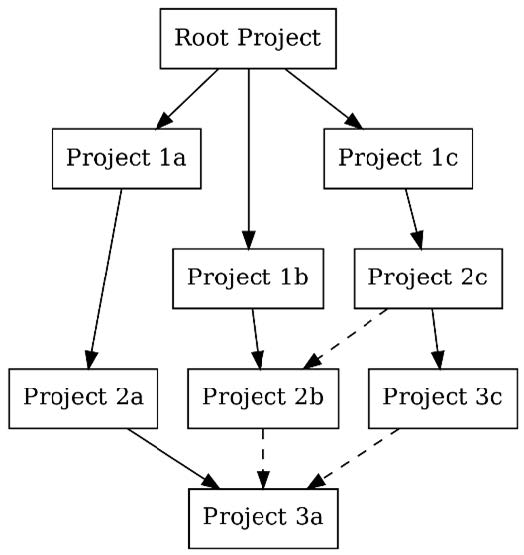
\includegraphics[width=0.8\textwidth]{content/3/chapter15/images/1.jpg}\\
Figure 15.1 – An example project hierarchy showing the various dependencies
\end{center}

Before migrating, the first thing to do is a thorough analysis of how the projects depend on each other and in what order they need to be built. Depending on the state of the project, the resulting graph might be quite large, so figuring out where to start might be a bit of a challenge. In reality, dependency graphs are often not as neat as the ones shown in this book. Whether it is easier to first disentangle the project and then move to CMake or move to CMake first and then disentangle the project depends on the actual situation. If projects are very large and complex, start by finding islands in the graph that are as self-contained as possible and start from there.

For complex, hierarchical projects, there are two general migration strategies to consider. One is a top-down approach, where the root project(s) are migrated and replaced first, and then the child projects are ordered by which one project has the least incoming dependencies. The second is a bottom-up approach, where the individual projects are migrated one by one, starting with the one that has the most incoming dependencies.

A top-down approach will have the benefit of ensuring the full project can be built, tested, and packaged with CMake early on, but it requires the existing build system to be integrated into CMake with ExternalProject. The downside of a top-down approach might be that, in the early stages, the resulting CMake project contains a lot of custom code to work with packages built by the old system. In practice, using a few temporary workarounds to include existing projects in the build is often the most pragmatic way of getting good results relatively quickly, and it partially mitigates the effort of maintaining two build systems for the same subprojects.

A bottom-up approach has the benefit that each library that is migrated to CMake can use dependencies that have already been migrated. The downside is that the root project can only be replaced once all the child projects are made buildable with CMake. Even though the projects are migrated from the bottom up, a good practice is for the root CMake project to be created early on. It lives side by side with the root project in the original build system. This allows you to put in external dependencies and install configuration and packaging instructions inside the new CMake project early on.

The following diagram illustrates how the top-down and bottom-up strategies look side by side. The numbers beside the boxes represent the order of migration:

\begin{center}
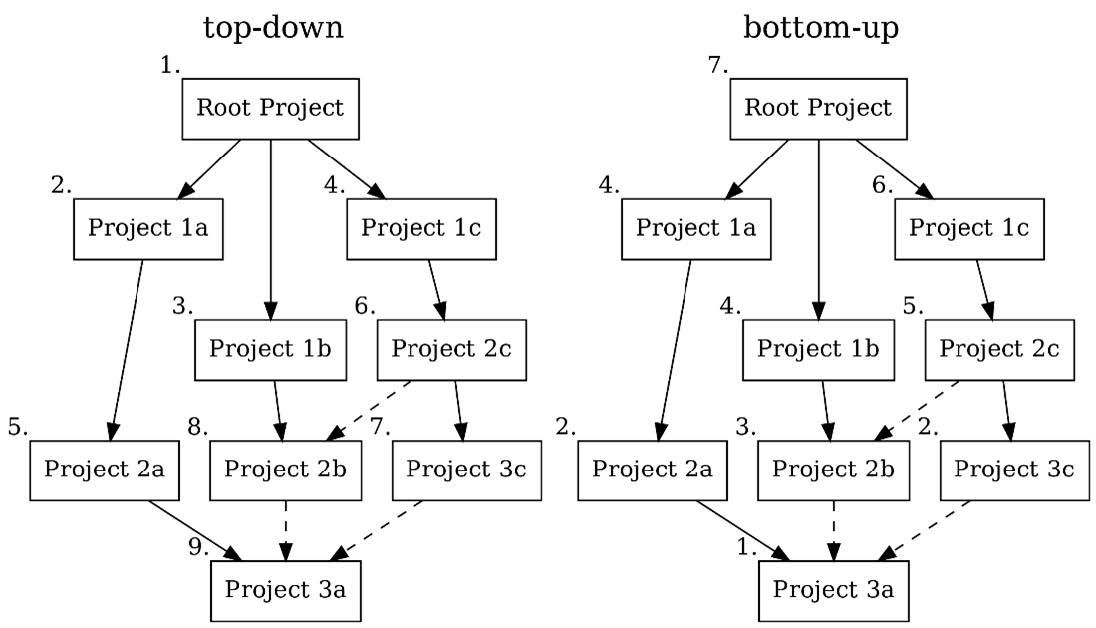
\includegraphics[width=0.8\textwidth]{content/3/chapter15/images/2.jpg}\\
Figure 15.2 – An example of migration orders
\end{center}

Apart from the overall migration strategy, another thing to consider is whether the project is going to be set up as a superbuild or as a regular project. When working with a top-down approach, a superbuild structure might be easier to migrate, as one of its benefits is that it is easier to integrate non-CMake projects by design. More information about superbuild structures can be found in Chapter 10, Handling Big Projects and Distributed Repositories in a Superbuild.

No matter whether you choose a top-approach down or a bottom-up approach for migrating the individual projects, the general strategy for migrating large projects will look similar to the following:

\begin{enumerate}
\item 
Analyze what the dependencies, project hierarchy, and deployment units are.

\item 
Decide on a migration strategy and whether a regular project structure or a superbuild is intended.

\item 
Create or migrate the root project and pull in all not-yet-converted projects using ExternalProject, FetchContent, or intermediate find modules if working with binary packages.

\item
Handle project-wide dependencies using CMake.

\item
Convert the child projects, one by one, into CMake, as described in the last section
of this chapter. If using intermediate find modules, replace them one by one:

\begin{enumerate}[label=\roman*]
\item
If desired, at this point, change the dependency handling to a package manager.

\item
Find common options and propagate them toward the root and create presets.
\end{enumerate}

\item
When migrating the children, organize the packaging in CMake if not already done.

\item
Clean up, reorganize the files and projects, improve performance, and more.
\end{enumerate}

Starting the migration by analyzing the existing project hierarchy and dependencies
will help you to set up a migration plan to communicate with all of the people involved.
Creating a visualization such as the one from earlier is often a good tool, although, for
very large projects, this can become quite a challenge in itself. Another important point to
bear in mind when creating the migration plan is to identify what is commonly deployed
together and which subproject has which frequency for releases. Projects that are rarely
changed and released might not be as critical to migrate as those that are frequently
touched and released. Identifying the deployment units is closely related to how projects
are packaged. Depending on how this is organized, it might not be possible to migrate the
packaging to CMake until all the projects have been migrated.

So far, we have mostly talked about subprojects, but while analyzing the existing structure,
it is important to recognize which of the subprojects are actually projects that should be
buildable as standalone and inside the full project context and which can be handled as
regular CMake targets that are rarely built outside the project context.

Creating the root CMakeLists.txt file will cover the basic project setup and include
the necessary modules such as FetchContent, CTest, CPack, and more. While not
directly in the CMakeLists.txt file, setting up toolchain files, build containers, or
sysroots for cross-compiling will also be done here. For large projects, often, the root
CMakeLists.txt file does not contain the targets directly. Rather, it includes them
either with add\_subdirectory or FetchContent, or in the case of a superbuild,
with ExternalProject. The root CMakeLists.txt file should have the
following structure:

\begin{enumerate}
\item 
The project definition and the minimum required version of CMake.

\item
Global properties and default variables such as the minimum language standard, the custom build types, and the search and module paths.

\item
Any modules and helper functions that are used project-wide.

\item
Project-wide external dependencies that are included via find\_package().

\item
The build targets and subprojects, possibly added with add\_subdirectory, FetchContent, or in the case of a superbuild, ExternalProject.

\item
Tests for the whole project. Typically, each subproject will have its own unit tests, but integration or system tests might be at the top level.

\item
Packaging instructions for CPack.
\end{enumerate}

Depending on the complexity of the definitions, it might help to put the handling of external dependencies, tests, and packaging into their own subdirectories to keep the CMake file short and concise. The external dependencies that are used project-wide might be large software frameworks, such as Qt or Boost, or small but common utility libraries that are used frequently.

For a top-down approach, the subprojects will be imported at the beginning and then migrated one by one. When using a bottom-up strategy, the build targets and subprojects will most likely be empty at the beginning and then become filled as the projects are migrated. When migrating the subprojects, keep your eyes open for common dependencies or build options that can be propagated to the root project or moved to presets.

Once all of the child projects have been migrated, typically, there are some maintenance tasks still open, such as organizing the packaging and orchestrating and grouping tests together. Also, it is not unusual for there to still be some clutter left in the CMake files after migrating everything, so having an extra round of cleaning up the centralizing functions will make sure that the migrated project is ready to use.

Often, migrating large projects is a challenge, especially if the build process is complicated and – unfortunately, as is frequently the case – lacks proper documentation. Software is built in many different ways, and the strategy described in this section tries to give a general approach. However, in the end, each migration will be unique in its own way. There are cases where the build system is so complex that the migration strategies described earlier are more of a hindrance than a help; for instance, including non-migrated projects into CMake is so difficult that a step-by-step migration might be more effort than just starting the build from scratch. Let's take a closer look at how the subprojects that use the original build system could be included when starting with a top-down approach.

\subsubsubsection{15.4.1\hspace{0.2cm}Integrating legacy projects when migrating top down}

For the top-down migration strategy, the existing projects are made available to CMake at the beginning. The easiest way is by using ExternalProject, regardless of whether a superbuild is intended or not. The imported targets can either be defined directly or with find modules. For regular projects, this is just an intermediate step to be able to build the full project relatively quickly and hand over control of the configuration and build order to CMake. The resulting CMake code might not look particularly nice, but the first goal is to get the root project building with CMake. However, be sure to clean it up, step by step, when migrating the subprojects. For regular projects that consist of a mono-repo or that pull in dependencies with Git submodules or similar, ExternalProject\_Add might omit downloading by specifying the SOURCE\_DIR property. The resulting CMake code for including the Autotools project might look like this:

\begin{lstlisting}[style=styleCMake]
include(ExternalProject)
set(ExtInstallDir ${CMAKE_CURRENT_BINARY_DIR}/install)
ExternalProject_Add(SubProjectXYZ_ext
	SOURCE_DIR ${CMAKE_CURRENT_LIST_DIR}/SubProjectXYZ/
	INSTALL_DIR ${ExtInstallDir}
	CONFIGURE_COMMAND <SOURCE_DIR>/configure --prefix <INSTALL_DIR>
	INSTALL_COMMAND make install
	BUILD_COMMAND make
)
add_library(SubProjectXYZ::SubProjectXYZ IMPORTED SHARED)
set_target_properties(SubProjectXYZ::SubProjectXYZ
	PROPERTIES IMPORTED_LOCATION " ${CMAKE_CURRENT_LIST_DIR}
		/SubProjectXYZ/lib/libSubProjectXYZ.so"
	INTERFACE_INCLUDE_DIRECTORIES "${CMAKE_CURRENT_LIST_DIR}
		/SubProjectXYZ/include"
	
	IMPORTED_LINK_INTERFACE_LANGUAGES "CXX"
)
...
add_dependencies(SomeTarget SubProjectXZY_ext)
target_link_libraries(SomeTarget SubProjectXYZ:: SubProjectXYZ)
\end{lstlisting}

As ExternalProject only makes the content available during build time, this approach only works for sub-projects that are already available in a local folder. Since they include directories of an imported target that have to exist at configuration time when using them in target\_link\_libraries, the exported location should point to the source directory rather than to the installation location of the external project.

\begin{tcolorbox}[colback=blue!5!white,colframe=blue!75!black,title=These Practices Are for Temporary Workarounds]
The practices using ExternalProject and FetchContent described here are meant for temporary workarounds to be able to include legacy projects in the CMake build while migrating. These are not good practices to use in a production environment. This pattern allows the use of the original build system and will provide an imported target to link against projects that have already been migrated. Whether the effort of creating such an intermediate project structure is justified by being able to build the full project with CMake early on, this has to be considered for each case separately.

If migrating from Microsoft Visual Studio instead of using ExternalProject, the include\_external\_msproject() function might be used to directly include the project files.
\end{tcolorbox}

With this, you should have all the concepts to migrate to CMake from another build system.


























